\chapter{Application Implementation}

\section{General Technologies and Frameworks}

As it is a web application, HTML, CSS and JavaScript were used for the client side of the application, although this was augmented with both \textit{JQuery} and \textit{Bootstrap} to ease the development of the Javascript and the CSS respectively. 

For the server side of the application, the code was written in python, using the \textit{Flask} framework and its integrated technologies. \textit{Flask} was used as it is easier to user then the alternative python frameworks and the developer has experience using it. python was also chosen for similar reasons and due to the fact that the developer likes it. The memory usage and speed of the various possible programming languages and frameworks was not considered. Ease of use and familiarity were the primary considerations. 

\section{Article Discovery}

For the article discovery portion of the application, the need was for a list of articles, from a variety of sources about a variety of topics. The solution that was found after some search on the internet, was \textit{Google News}.

\textit{Google News} provides several lists of recent articles from different sources divided in different topics, additionally, each of these lists is provided in an RSS feed XML file, a format that allows the code to be written for both URL and title extraction with minimal effort, both on the parts of the developer and the machine life time.

The categories provided by the \textit{Google News} RSS feeds were usable, but overall they were fairly common news categories. On the plus side, these categories are recognisable, on the down side, these categories are not customisable, however, the categories were pre-selected, saving time on artificial category creation, the end user can just selected one of them. 

There were alternatives to the \textit{Google News} RSS feeds that were examined, primarily \textit{NewsAPI}. However this was found to be lacking for two reasons. Primarily, this API would list content, where the primary means of communication was not text. Comics and other image based got added to the lists being provided by the API. As the parser and the gloss system relied on the content being text based and there was no easy way to distinguish being text based content and image based content. The other more minor reason that \textit{NewsAPI} was disregarded was because it was more difficult to categorise the articles, whereas the \textit{Google News} RSS feeds provided pre-created categories, to save time on both filtering out image-based content and the categorisation of articles, the decision was made to use the \textit{Google News} RSS feeds. 

The end result of this is an application is that the articles being listed in the article selection view are pulled from the Google News RSS feed that corresponds to the category selected by the end user.

\section{Article Difficulty Rating}

The difficulty rating of the article is calculated using two things, the article text as well as the user's experience level. The user's experience level is obtained from the form the user submitted at the start, while the article text needs to be extracted from the article web page and then analysed.

To extract and then analyse the article, two technologies are used. The first is an article scraping python library called \textit{Newspaper}, the purpose of it is to extract the raw article text from the article web page, making the analysis of it easier. Analysis of the article text is then done through another python library called \textit{SpaCy}, which is a parts-of-speech tagging library, with some additional advanced features, pretty much all the analysis is performed when the article text is parsed into the library, meaning that library provides a bunch of information about the text.

Once the article text has been extracted and analysed, it's readability index needs to be calculated, this is done using the Erste Wiener Sachetextformel as described in \textcite{bamberger1984}. The WSTF formula was chosen over the FRE formula because the WSTF formula has a smaller output range. This smaller output range allowed for two things the first was easier mapping onto the user experience level as well as a better understanding of the approximate level of each individual number, as those number correspond directly with the German school years. 

Once the readability score is calculated, it needs to be mapped, using the user experience level onto the difficulty ratings, a simple linear map was chosen for this, the mapping system can be seen in table \ref{tbl:ratings}.

\begin{table}
\centering
\caption{Comparison of Translation Software}
\label{tbl:ratings}
\begin{tabu} to \textwidth{|l|c|c|c|c|c|c|c|}
\hline
\textbf{Rating} & \textbf{SL}      & \textbf{L}       & \textbf{ZL}   & \textbf{M}    & \textbf{ZS}   & \textbf{S}  & \textbf{SS}   \\ \hline
Beginner                  & $ r < 2 $ & $ 2 \leq r < 3 $ & $ 3 \leq r < 4 $ & $ 4 \leq r < 5 $ & $ 5 \leq r < 6 $  & $ 6 \leq r < 7 $ & $ 7 \leq r $    \\ \hline
Intermediate              & $ r < 4 $ & $ 4 \leq r < 5 $ & $ 5 \leq r < 6 $ & $ 6 \leq r < 7 $ & $ 7 \leq r < 8 $  & $ 8 \leq r < 9 $ & $ 9 \leq r $    \\ \hline
Advanced                  & $ r < 6 $ & $ 6 \leq r < 7 $ & $ 7 \leq r < 8 $ & $ 8 \leq r < 9 $ & $ 9 \leq r < 10 $  & $ 10 \leq r < 11 $ & $ 11 \leq r $    \\ \hline
Near Fluent             & $ r < 8 $ & $ 8 \leq r < 9 $ & $ 9 \leq r < 10 $ & $ 10 \leq r < 11 $ & $ 11 \leq r < 12 $  & $ 12 \leq r < 13 $ & $ 13 \leq r $    \\ \hline
\end{tabu}
\end{table}

The primary idea behind these ratings was that a user who was less experienced with German would find have a lower threshold for articles that they find difficult. To do this it was decided that near fluent user would be able to read with some confidence articles with a WSTF score of 10 which corresponds to a native speaker who is 15/16 years old. The rest of the mapping were calculated then using this as baseline. 

More complex ideas for mapping were experimented with, including ones that used machine learning systems, however these ideas were eventually abandoned due to the fact that they were to complex to be implemented in the limited time available. 

\section{Displaying the Article}

Once the users has selected an article, they are then presented with the content of that article. The actual job of presenting this article was fairly easy as the was majority of this work (the extraction and parsing of the article's content) had already been done by \textit{newspaper} and \textit{SpaCy}.  \textit{SpaCy's} method of presenting the parsed article is as a series of tags, each representing a part of speech. This leaves very little difficulty in presenting the article, the tags are iterated through as if they were a list. Words are wrapped in span elements tags for later use, punctuation is skipped over and paragraph breaks end the current paragraph and start a new one. In addition these span tags have data attributes storing the parts of speech tags and root word. This results in a html document that appears similar to listing \ref{lst:html}.

\begin{lstlisting}[language=HTML, caption=Example HTML Code, label=lst:html, breaklines=true]
<p>
	<span class="word" data-lemma="Der" data-tag="ART" data-pos="DET">Der</span>
	<span class="word" data-lemma="Index" data-tag="NN" data-pos="NOUN">Index</span>
	<span class="word" data-lemma="der" data-tag="ART" data-pos="DET">der</span>
	<span class="word" data-lemma="30" data-tag="CARD" data-pos="NUM">30</span>
	<span class="word" data-lemma="groß" data-tag="ADJA" data-pos="ADJ">größten</span>
	<span class="word" data-lemma="Aktiengesellschaften" data-tag="NN" data-pos="NOUN">Aktiengesellschaften</span>
	<span class="word" data-lemma="steigen" data-tag="VVFIN" data-pos="VERB">stieg</span>
	<span class="word" data-lemma="heute" data-tag="ADV" data-pos="ADV">heute</span>
	<span class="word" data-lemma="zeitweise" data-tag="ADV" data-pos="ADV">zeitweise</span>
	<span class="word" data-lemma="bis" data-tag="APPR" data-pos="ADP">bis</span>
	<span class="word" data-lemma="auf" data-tag="ADV" data-pos="ADV">auf</span>
	<span class="word" data-lemma="12.524,97" data-tag="CARD" data-pos="NUM">12.524,97</span>
	<span class="word" data-lemma="punkten" data-tag="NN" data-pos="NOUN">Punkte</span>
	,
	<span class="word" data-lemma="entsprechen" data-tag="ADJD" data-pos="ADJ">entsprechend</span>
	<span class="word" data-lemma="einer" data-tag="ART" data-pos="DET">einem</span>
	<span class="word" data-lemma="gewinnen" data-tag="NN" data-pos="NOUN">Gewinn</span>
	<span class="word" data-lemma="von" data-tag="APPR" data-pos="ADP">von</span>
	<span class="word" data-lemma="0,13" data-tag="CARD" data-pos="NUM">0,13</span>
	<span class="word" data-lemma="Prozent" data-tag="NN" data-pos="NOUN">Prozent</span>
	.
</p>

\end{lstlisting}

The html produced by this was functional, although there was a bug to do with the generation of excess whitespace, which was removed from listing \ref{lst:html} to make sure the code was readable. 

\section{Gloss Creation}

The client side method for creating the gloss is done through AJAX, the javascript for this can be seen in listing \ref{lst:gloss}.



\begin{lstlisting}[caption={[Gloss Javascript] Javascript/JQuery code for obtaining gloss content from the server and then inserting it into the web page.}, label=lst:gloss, language=javascript, float]
$('.word').on('click', function (event) {
	var e = event.target;
	var data = e.dataset;
	data.word = e.textContent;
	$.ajax({
		url: "/dict",
		type: 'POST',
		data: data,
		success: function (result) {
			popupEntry(result);
		}
	});
});

function popupEntry(entry) {
	var entryList = document.getElementById("dict-entries");
	entryList.insertAdjacentHTML('beforeend', entry);
}

\end{lstlisting}

This code is simple, when one of the words is click, an AJAX event is fired. It requests the gloss item from the application, and upon return inserts the gloss item at the end of the marginal gloss.

Upon recieve such an gloss request, the server side python code will then generate an return a pre-formatted gloss. This allowed for the client side code to be kept as simple as possible.

\subsection{Translation Lookup}

For the translation section of the gloss creation, various possibilities were considered, These included online translation services such as \textit{Google Cloud Translate} and \textit{Microsoft Translator}, raw datasets such as the \textit{DictCC dataset} and Dictionary APIs such as the \textit{Oxford Dictionaries API} and the \textit{Collins Dictionary API}. 

The technology that would be used in the project would have to:
\begin{itemize}
\item Be able to translate single words from to English
\item Provide Lexical information of those words
\item Be allowed for the content to be hosted and provided through a web interface
\item Be available for less than \pounds150 total
\end{itemize}

The five technologies cited above were checked against these criteria and the results are show in Table \ref{tbl:comp}

\begin{table}
\centering
\caption[Comparison of Translation Software]{Comparison of various translation solutions to see whether or not they fulfil the criteria of the application. }
\label{tbl:comp}
\begin{tabu} to \textwidth{|X[c]|X[c]|X[c]|X[c]|X[c]|}
\hline
\textbf{Product}        & \textbf{German to English Translations} & \textbf{Lexical Information} & \textbf{Allowed Online} & \textbf{Less Than \pounds150  (total)} \\ \hline
Google Cloud Translate  & Yes                                     & No                           & Yes                     & No                               \\ \hline
Microsoft Translator    & Yes                                     & No                           & Yes                     & No                               \\ \hline
Dict.cc Dataset         & Yes                                     & Yes                          & No                      & Yes                              \\ \hline
Oxford Dictionaries API & Yes                                     & Yes                          & Yes                     & Yes                              \\ \hline
Collins Dictionary API  & Yes                                     & Yes                          & Yes                     & No                               \\ \hline
\end{tabu}
\end{table}

As the \textit{Oxford Dictionaries API} was the only technology to clear all four criteria, the decision was made to used it for development of the application, however other technologies were used in testing the resulting code.

\textit{Oxford Dictionaries API} is a REST API where two calls are required to get the desired information. The first, gets the translations of the root words, at the same time this is used to check if a word is the dictionary, the second call, which is made if a translation is found is to get the reasons why that particular mutation from the root occurred.  The process is illustrated in the systems flow diagram in figure \ref{fig:odsf}

\begin{figure}
	\caption{Systems Flow Diagram of the Oxford Dictionaries API}
	\label{fig:odsf}
	\begin{center}
	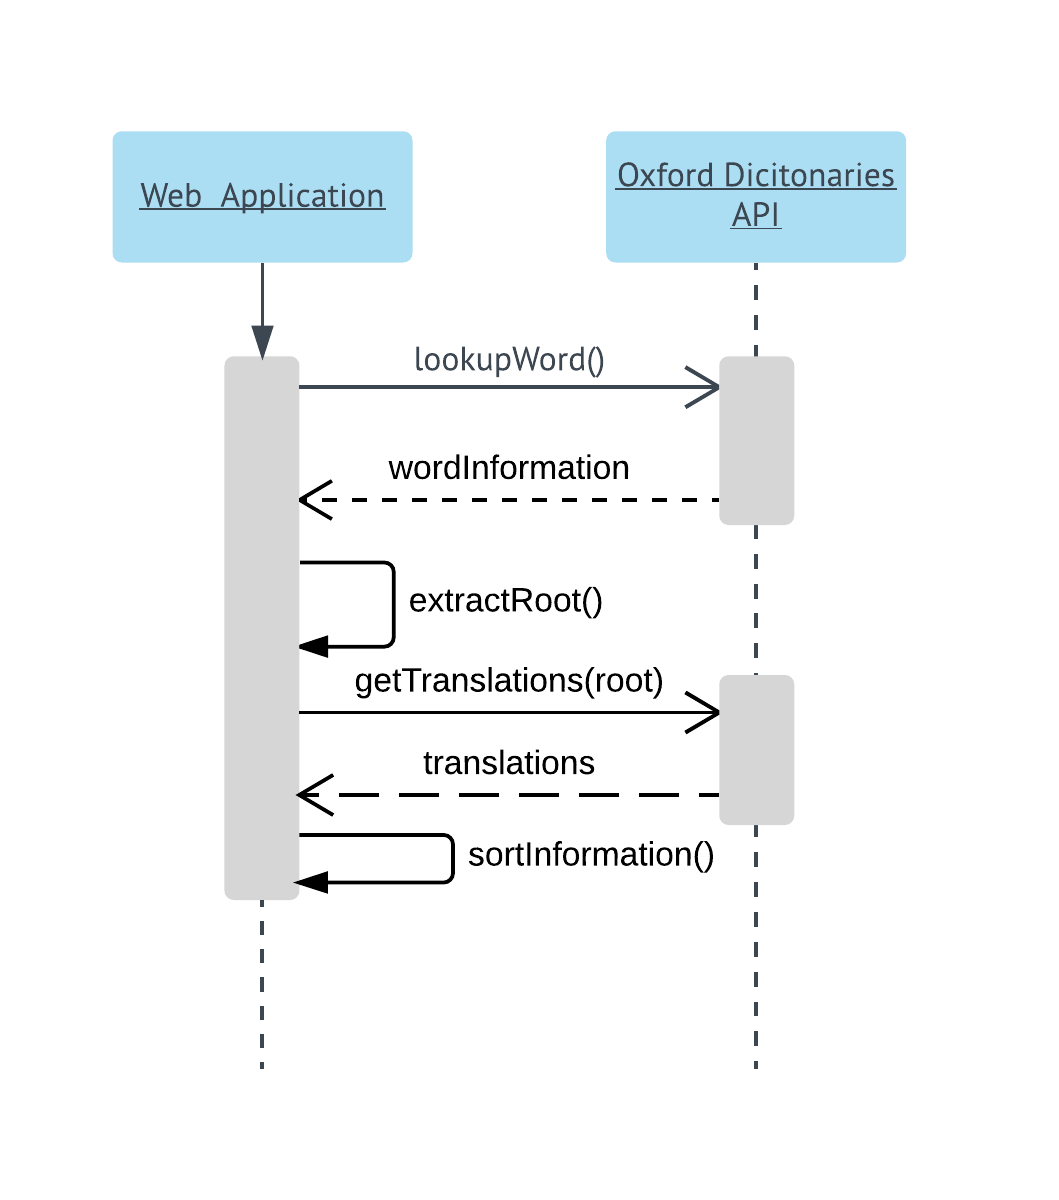
\includegraphics[width=0.7\textwidth]{Graphics/SystemsFlowOxford}
\end{center}
\end{figure}

On the first call, the root word, as provided by \textit{SpaCy}, gets its translations looked up. If one or more translation is discovered, the second call gets made, extracting the grammatical information about why the root was transformed into it's current form. Both this grammatical information and the tag explanation from \textit{SpaCy} were used in the final gloss. A breakdown of where the various parts of the gloss are sourced from can be seen in figure 

